% 5-minute talk by Longtao Jiang: continual learning, Q2–Q3. Script: script_longtao.md
\documentclass[aspectratio=169,11pt]{beamer}
% Shared preamble and frames for the three 5-minute talks.
% Each talk sets \presenter{...} before % Shared preamble and frames for the three 5-minute talks.
% Each talk sets \presenter{...} before % Shared preamble and frames for the three 5-minute talks.
% Each talk sets \presenter{...} before \input{common}.
\usepackage{amsmath,amssymb}
\usepackage{booktabs}
\usepackage{xcolor}
\usetheme{MBZUAI}
\graphicspath{{assets/}{../figs/}}
\setbeamertemplate{navigation symbols}{}

\newcommand{\lam}{\lambda}
\newcommand{\strong}[1]{\textcolor{mbzuai-navy}{\textbf{#1}}}
\newcommand{\good}[1]{\textcolor{green!45!black}{\textbf{#1}}}
\newcommand{\bad}[1]{\textcolor{red!65!black}{\textbf{#1}}}

% ── Team and roles: edit here, all three decks update ─────────────────────
\newcommand{\roleJH}{Problem and setup; score cache and data pipeline; Q1 analysis; overall study (Q1--Q4)}
\newcommand{\roleLJ}{Continual learning experiments and analysis (Q2--Q3)}
\newcommand{\roleMA}{Downstream question-answering evaluation (Q4)}

\title[Fusion Weight for Keyframe Search]{Should the Fusion Weight Change with the Question?}
\institute[MBZUAI]{CV805 Course Project \\ Mohamed bin Zayed University of Artificial Intelligence}
\date{\today}
\titlelogos{assets/logo_dark.pdf}
\footleft{Should the Fusion Weight Change with the Question?}
\footright{\insertframenumber{} / \inserttotalframenumber}

% Team slide; #1 = JH, LJ or MA, the presenter's row is highlighted.
\usepackage{etoolbox}
\newcommand{\teamrow}[4]{% #1 key, #2 presenter key, #3 name, #4 role
  \ifstrequal{#1}{#2}%
    {\textbf{\textcolor{mbzuai-navy}{#3}} & \textbf{\textcolor{mbzuai-navy}{#4}} & \textcolor{mbzuai-dark-sand}{\textbf{this talk}}}%
    {\textcolor{mbzuai-subtle}{#3} & \textcolor{mbzuai-subtle}{#4} & }}
\newcommand{\teamframe}[1]{%
\begin{frame}{Team and my part}
  \centering
  \renewcommand{\arraystretch}{1.6}
  \begin{tabular}{p{0.27\textwidth}p{0.52\textwidth}p{0.11\textwidth}}
    \toprule
    Member & Main contribution & \\
    \midrule
    \teamrow{JH}{#1}{Jianxiang He}{\roleJH} \\
    \teamrow{LJ}{#1}{Longtao Jiang}{\roleLJ} \\
    \teamrow{MA}{#1}{Makhmud Assentay}{\roleMA} \\
    \bottomrule
  \end{tabular}
\end{frame}}

% Context frame used by every talk: VSI, the weight, and the example.
\newcommand{\contextframe}{%
\begin{frame}{Background: two clues, one weight}
  \begin{columns}[c,onlytextwidth]
    \begin{column}{0.47\textwidth}
      \small
      A VLM can only look at \strong{about 8 frames} of a long video, so we must pick them well.\\[2mm]
      VSI scores every second with two clues:
      \begin{itemize}
        \item \strong{Visual}: do the question's objects appear?
        \item \strong{Subtitle}: does the subtitle match the question?
      \end{itemize}
      \[ S(t) = (1-\lam)\,\text{visual}(t) + \lam\,\text{subtitle}(t) \]
      and keeps the top 8 seconds. VSI uses \strong{$\lam=0.3$ for every question}.
    \end{column}
    \begin{column}{0.5\textwidth}
      \centering
      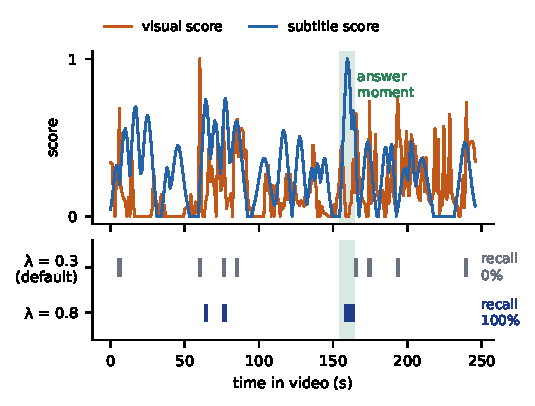
\includegraphics[width=\linewidth]{f01_teaser.pdf}\\
      {\scriptsize Real example: $\lam=0.3$ \bad{misses} the answer moment (green), $\lam=0.8$ \good{hits} it.}
    \end{column}
  \end{columns}
\end{frame}}

\newcommand{\titleframe}{%
{\setbeamertemplate{footline}{}\setbeamertemplate{frametitle}{}
\begin{frame}[t]\titlepage\end{frame}}}

\newcommand{\thankframe}{%
{\setbeamertemplate{footline}{}\setbeamertemplate{frametitle}{}
\begin{frame}[t]\mbzuaiThankYou\end{frame}}}
.
\usepackage{amsmath,amssymb}
\usepackage{booktabs}
\usepackage{xcolor}
\usetheme{MBZUAI}
\graphicspath{{assets/}{../figs/}}
\setbeamertemplate{navigation symbols}{}

\newcommand{\lam}{\lambda}
\newcommand{\strong}[1]{\textcolor{mbzuai-navy}{\textbf{#1}}}
\newcommand{\good}[1]{\textcolor{green!45!black}{\textbf{#1}}}
\newcommand{\bad}[1]{\textcolor{red!65!black}{\textbf{#1}}}

% ── Team and roles: edit here, all three decks update ─────────────────────
\newcommand{\roleJH}{Problem and setup; score cache and data pipeline; Q1 analysis; overall study (Q1--Q4)}
\newcommand{\roleLJ}{Continual learning experiments and analysis (Q2--Q3)}
\newcommand{\roleMA}{Downstream question-answering evaluation (Q4)}

\title[Fusion Weight for Keyframe Search]{Should the Fusion Weight Change with the Question?}
\institute[MBZUAI]{CV805 Course Project \\ Mohamed bin Zayed University of Artificial Intelligence}
\date{\today}
\titlelogos{assets/logo_dark.pdf}
\footleft{Should the Fusion Weight Change with the Question?}
\footright{\insertframenumber{} / \inserttotalframenumber}

% Team slide; #1 = JH, LJ or MA, the presenter's row is highlighted.
\usepackage{etoolbox}
\newcommand{\teamrow}[4]{% #1 key, #2 presenter key, #3 name, #4 role
  \ifstrequal{#1}{#2}%
    {\textbf{\textcolor{mbzuai-navy}{#3}} & \textbf{\textcolor{mbzuai-navy}{#4}} & \textcolor{mbzuai-dark-sand}{\textbf{this talk}}}%
    {\textcolor{mbzuai-subtle}{#3} & \textcolor{mbzuai-subtle}{#4} & }}
\newcommand{\teamframe}[1]{%
\begin{frame}{Team and my part}
  \centering
  \renewcommand{\arraystretch}{1.6}
  \begin{tabular}{p{0.27\textwidth}p{0.52\textwidth}p{0.11\textwidth}}
    \toprule
    Member & Main contribution & \\
    \midrule
    \teamrow{JH}{#1}{Jianxiang He}{\roleJH} \\
    \teamrow{LJ}{#1}{Longtao Jiang}{\roleLJ} \\
    \teamrow{MA}{#1}{Makhmud Assentay}{\roleMA} \\
    \bottomrule
  \end{tabular}
\end{frame}}

% Context frame used by every talk: VSI, the weight, and the example.
\newcommand{\contextframe}{%
\begin{frame}{Background: two clues, one weight}
  \begin{columns}[c,onlytextwidth]
    \begin{column}{0.47\textwidth}
      \small
      A VLM can only look at \strong{about 8 frames} of a long video, so we must pick them well.\\[2mm]
      VSI scores every second with two clues:
      \begin{itemize}
        \item \strong{Visual}: do the question's objects appear?
        \item \strong{Subtitle}: does the subtitle match the question?
      \end{itemize}
      \[ S(t) = (1-\lam)\,\text{visual}(t) + \lam\,\text{subtitle}(t) \]
      and keeps the top 8 seconds. VSI uses \strong{$\lam=0.3$ for every question}.
    \end{column}
    \begin{column}{0.5\textwidth}
      \centering
      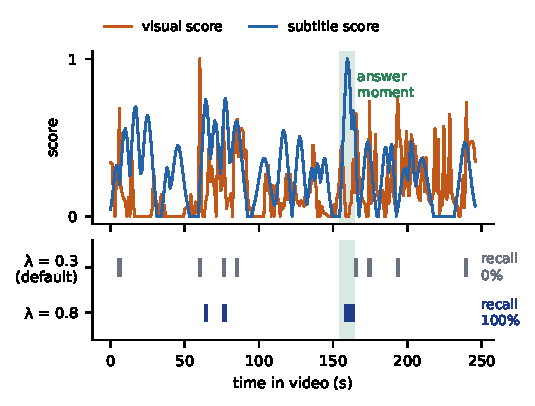
\includegraphics[width=\linewidth]{f01_teaser.pdf}\\
      {\scriptsize Real example: $\lam=0.3$ \bad{misses} the answer moment (green), $\lam=0.8$ \good{hits} it.}
    \end{column}
  \end{columns}
\end{frame}}

\newcommand{\titleframe}{%
{\setbeamertemplate{footline}{}\setbeamertemplate{frametitle}{}
\begin{frame}[t]\titlepage\end{frame}}}

\newcommand{\thankframe}{%
{\setbeamertemplate{footline}{}\setbeamertemplate{frametitle}{}
\begin{frame}[t]\mbzuaiThankYou\end{frame}}}
.
\usepackage{amsmath,amssymb}
\usepackage{booktabs}
\usepackage{xcolor}
\usetheme{MBZUAI}
\graphicspath{{assets/}{../figs/}}
\setbeamertemplate{navigation symbols}{}

\newcommand{\lam}{\lambda}
\newcommand{\strong}[1]{\textcolor{mbzuai-navy}{\textbf{#1}}}
\newcommand{\good}[1]{\textcolor{green!45!black}{\textbf{#1}}}
\newcommand{\bad}[1]{\textcolor{red!65!black}{\textbf{#1}}}

% ── Team and roles: edit here, all three decks update ─────────────────────
\newcommand{\roleJH}{Problem and setup; score cache and data pipeline; Q1 analysis; overall study (Q1--Q4)}
\newcommand{\roleLJ}{Continual learning experiments and analysis (Q2--Q3)}
\newcommand{\roleMA}{Downstream question-answering evaluation (Q4)}

\title[Fusion Weight for Keyframe Search]{Should the Fusion Weight Change with the Question?}
\institute[MBZUAI]{CV805 Course Project \\ Mohamed bin Zayed University of Artificial Intelligence}
\date{\today}
\titlelogos{assets/logo_dark.pdf}
\footleft{Should the Fusion Weight Change with the Question?}
\footright{\insertframenumber{} / \inserttotalframenumber}

% Team slide; #1 = JH, LJ or MA, the presenter's row is highlighted.
\usepackage{etoolbox}
\newcommand{\teamrow}[4]{% #1 key, #2 presenter key, #3 name, #4 role
  \ifstrequal{#1}{#2}%
    {\textbf{\textcolor{mbzuai-navy}{#3}} & \textbf{\textcolor{mbzuai-navy}{#4}} & \textcolor{mbzuai-dark-sand}{\textbf{this talk}}}%
    {\textcolor{mbzuai-subtle}{#3} & \textcolor{mbzuai-subtle}{#4} & }}
\newcommand{\teamframe}[1]{%
\begin{frame}{Team and my part}
  \centering
  \renewcommand{\arraystretch}{1.6}
  \begin{tabular}{p{0.27\textwidth}p{0.52\textwidth}p{0.11\textwidth}}
    \toprule
    Member & Main contribution & \\
    \midrule
    \teamrow{JH}{#1}{Jianxiang He}{\roleJH} \\
    \teamrow{LJ}{#1}{Longtao Jiang}{\roleLJ} \\
    \teamrow{MA}{#1}{Makhmud Assentay}{\roleMA} \\
    \bottomrule
  \end{tabular}
\end{frame}}

% Context frame used by every talk: VSI, the weight, and the example.
\newcommand{\contextframe}{%
\begin{frame}{Background: two clues, one weight}
  \begin{columns}[c,onlytextwidth]
    \begin{column}{0.47\textwidth}
      \small
      A VLM can only look at \strong{about 8 frames} of a long video, so we must pick them well.\\[2mm]
      VSI scores every second with two clues:
      \begin{itemize}
        \item \strong{Visual}: do the question's objects appear?
        \item \strong{Subtitle}: does the subtitle match the question?
      \end{itemize}
      \[ S(t) = (1-\lam)\,\text{visual}(t) + \lam\,\text{subtitle}(t) \]
      and keeps the top 8 seconds. VSI uses \strong{$\lam=0.3$ for every question}.
    \end{column}
    \begin{column}{0.5\textwidth}
      \centering
      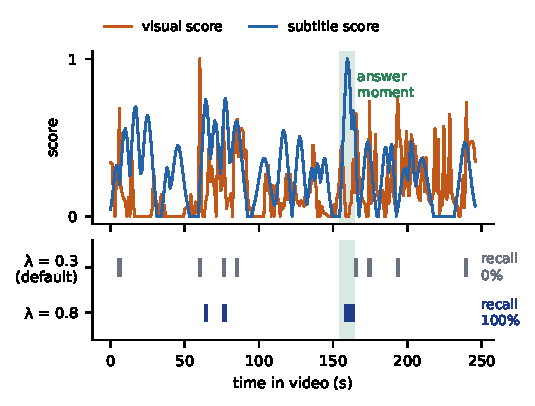
\includegraphics[width=\linewidth]{f01_teaser.pdf}\\
      {\scriptsize Real example: $\lam=0.3$ \bad{misses} the answer moment (green), $\lam=0.8$ \good{hits} it.}
    \end{column}
  \end{columns}
\end{frame}}

\newcommand{\titleframe}{%
{\setbeamertemplate{footline}{}\setbeamertemplate{frametitle}{}
\begin{frame}[t]\titlepage\end{frame}}}

\newcommand{\thankframe}{%
{\setbeamertemplate{footline}{}\setbeamertemplate{frametitle}{}
\begin{frame}[t]\mbzuaiThankYou\end{frame}}}

\subtitle{Part 2: Can Continual Learning Learn the Weight? (Q2--Q3)}
\author[Longtao Jiang]{Longtao Jiang \\ \small with Jianxiang He and Makhmud Assentay}
\footmid{Longtao Jiang}

\begin{document}
\titleframe
\teamframe{LJ}
\contextframe

\begin{frame}{My part: learning the weight}
  \begin{columns}[T,onlytextwidth]
    \begin{column}{0.5\textwidth}
      \begin{itemize}
        \item The best $\lam$ differs by question type: text questions want \strong{0.8--0.9}, visual questions \strong{$\le$0.3}.
        \item Idea: a \strong{small predictor} outputs $\lam$ for each question.
        \item New question types keep arriving, so it learns them \strong{one after another} without forgetting: \strong{continual learning}.
      \end{itemize}
    \end{column}
    \begin{column}{0.46\textwidth}
      \begin{block}{My part (Q2--Q3)}
        \begin{itemize}
          \item[Q2] Can continual learning learn $\lam$? Does it forget?
          \item[Q3] If the gain is small, why?
        \end{itemize}
      \end{block}
      \small I ran and analysed the continual learning experiments: 6 methods $\times$ 3 orders $\times$ 3 seeds.
    \end{column}
  \end{columns}
\end{frame}

\begin{frame}{Setup: four types in sequence}
  \small
  \begin{columns}[T,onlytextwidth]
    \begin{column}{0.48\textwidth}
      \strong{Tasks} (learned in order): T1 text perception, T2 visual perception, T3 text relation, T4 visual relation (753 questions)\\[1mm]
      \strong{Predictor}: small 2-layer network, 54 inputs from the two score curves\\[1mm]
      \strong{Methods}: Naive (just keep training), EWC (protect important weights), LwF (imitate the old model), ER (replay old questions), kNN, Joint (train on everything; reference)
    \end{column}
    \begin{column}{0.48\textwidth}
      \strong{Metrics}
      \begin{itemize}
        \item ACC: final recall@8 averaged over the 4 types
        \item FM (forgetting): how far old types drop from their best
      \end{itemize}
      \strong{Baselines}
      \begin{itemize}
        \item default $\lam=0.3$
        \item \textbf{one $\lam$ tuned on the training set}
        \item one $\lam$ per type; oracle
      \end{itemize}
    \end{column}
  \end{columns}
\end{frame}

\begin{frame}{Q2: results over 9 runs}
  \begin{columns}[c,onlytextwidth]
    \begin{column}{0.55\textwidth}
      \centering\small
      \begin{tabular}{lccc}
        \toprule
        Method & ACC $\uparrow$ & FM $\downarrow$ & vs.\ tuned \\
        \midrule
        Default $\lam=0.3$ & 0.617 & -- & $-$4.5 \\
        \rowcolor{mbzuai-light-gray}
        One tuned $\lam$ & 0.662 & -- & -- \\
        One $\lam$ per type & 0.677 & -- & +1.4 \\
        \midrule
        Naive & 0.656 & 0.029 & $-$0.7 \\
        EWC & 0.662 & 0.023 & $-$0.1 \\
        \rowcolor{mbzuai-light-gray}
        LwF & \textbf{0.668} & \textbf{0.015} & +0.6 \\
        ER & 0.660 & 0.021 & $-$0.3 \\
        Joint (ref.) & \textbf{0.668} & \textbf{0.015} & +0.6 \\
        kNN & 0.645 & 0.005 & $-$1.7 \\
        \bottomrule
      \end{tabular}
    \end{column}
    \begin{column}{0.42\textwidth}
      \begin{itemize}
        \item Every method beats the default by \good{4--5 points}, in \strong{9/9} runs
        \item Against \strong{one tuned $\lam$}: best gain only \bad{+0.6}
        \item None reaches one $\lam$ per type
      \end{itemize}
    \end{column}
  \end{columns}
\end{frame}

\begin{frame}{Q2: the right baseline matters}
  \centering
  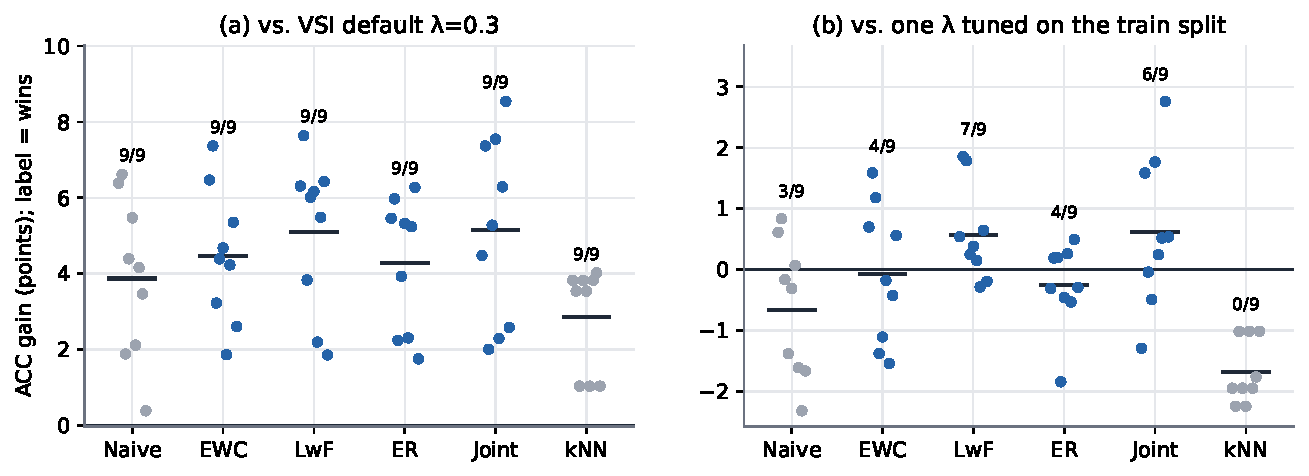
\includegraphics[width=0.88\textwidth]{f10_paired.pdf}
  \par\vspace{1mm}
  \small Each dot = one run. (a) vs.\ default: always better. (b) vs.\ one tuned $\lam$: \strong{about even}.
\end{frame}

\begin{frame}{Q3: one weight for every type}
  \centering
  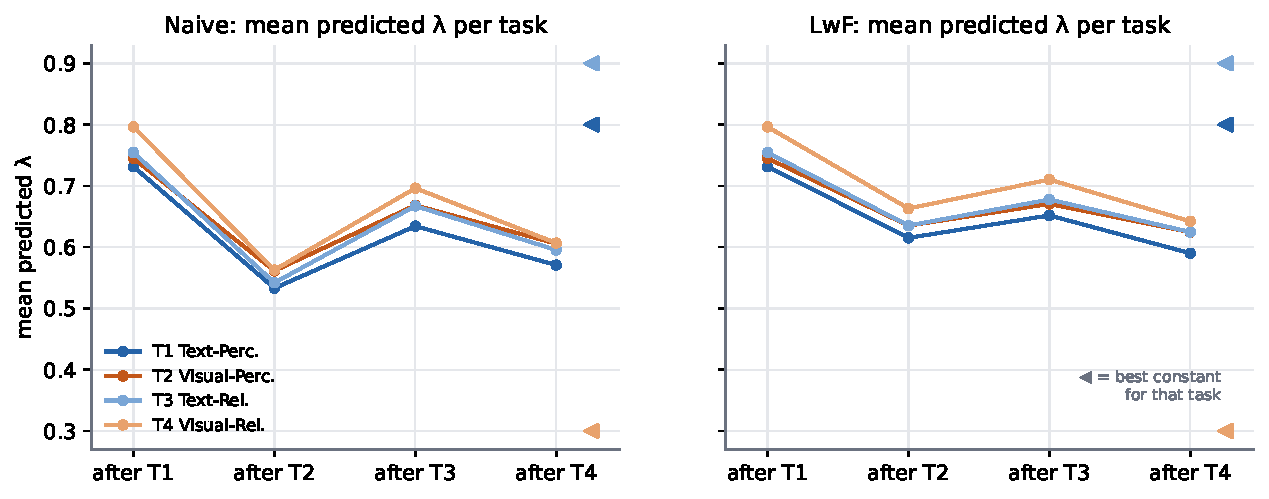
\includegraphics[width=0.84\textwidth]{f12_lambda_rounds.pdf}
  \par\vspace{1mm}
  \small Average predicted $\lam$ per type after each stage; triangles = best $\lam$ for that type.\\
  The lines overlap at $\approx$0.6: a \strong{better global value}, not \bad{different values per type}.
\end{frame}

\begin{frame}{Q3: why, and forgetting}
  \begin{columns}[T,onlytextwidth]
    \begin{column}{0.48\textwidth}
      \begin{block}{Why it cannot learn the differences}
        \begin{enumerate}
          \item \textbf{Sparse signal}: 62\% of questions give the same result for every $\lam$.
          \item \textbf{No type information}: inputs only describe the score curves; adding the question text overfits.
        \end{enumerate}
      \end{block}
    \end{column}
    \begin{column}{0.48\textwidth}
      \begin{exampleblock}{Why forgetting is small}
        All types get similar weights, so a new type overwrites little. LwF and Joint forget about \strong{half} as much as Naive (0.015 vs.\ 0.029), but only in 6/9 runs.
      \end{exampleblock}
    \end{column}
  \end{columns}
\end{frame}

\begin{frame}{Takeaways from Q2--Q3}
  \begin{enumerate}
    \item Continual learning \strong{beats the default} weight in every run, by 4--5 points.
    \vspace{2mm}
    \item But it only \strong{ties a tuned constant}, because it collapses to one weight for all question types.
    \vspace{2mm}
    \item Forgetting is \strong{small} for every method; anti-forgetting methods help only weakly.
    \vspace{2mm}
    \item Next: give the predictor the question type, or start from one $\lam$ per type and learn per-question corrections.
  \end{enumerate}
\end{frame}

\thankframe

% ════════════════════════════ backup for Q&A ════════════════════════════
\appendix

\begin{frame}{Backup: training details}
  \small
  \begin{itemize}
    \item Outputs probabilities over 11 values $\lam\in\{0,0.1,\dots,1\}$; uses their \strong{weighted average} $\bar\lam$.
    \item ``Best $\lam$'' labels carry little signal (most questions are flat), so we train it to rank the annotated seconds high:
    \[ \mathcal{L} = -\log \sum_{t\in\text{GT}} \operatorname{softmax}\big(S_{\bar\lam}/\tau\big)_t,\quad \tau=0.1 \]
    \item 50 epochs per type, Adam, lr $10^{-3}$, batch 64. EWC weight 400; LwF temperature 2; ER buffer 200; kNN $k=5$.
    \item Inputs standardized with the \strong{first} type's statistics only (no leakage).
  \end{itemize}
\end{frame}

\begin{frame}{Backup: where the gain is}
  \centering
  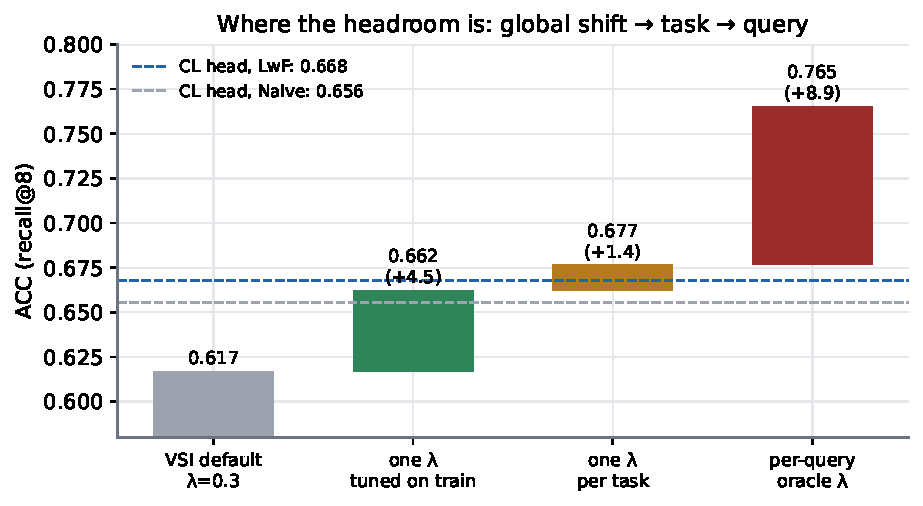
\includegraphics[height=0.72\textheight]{f16_decomp.pdf}
\end{frame}

\begin{frame}{Backup: recall matrices}
  \centering
  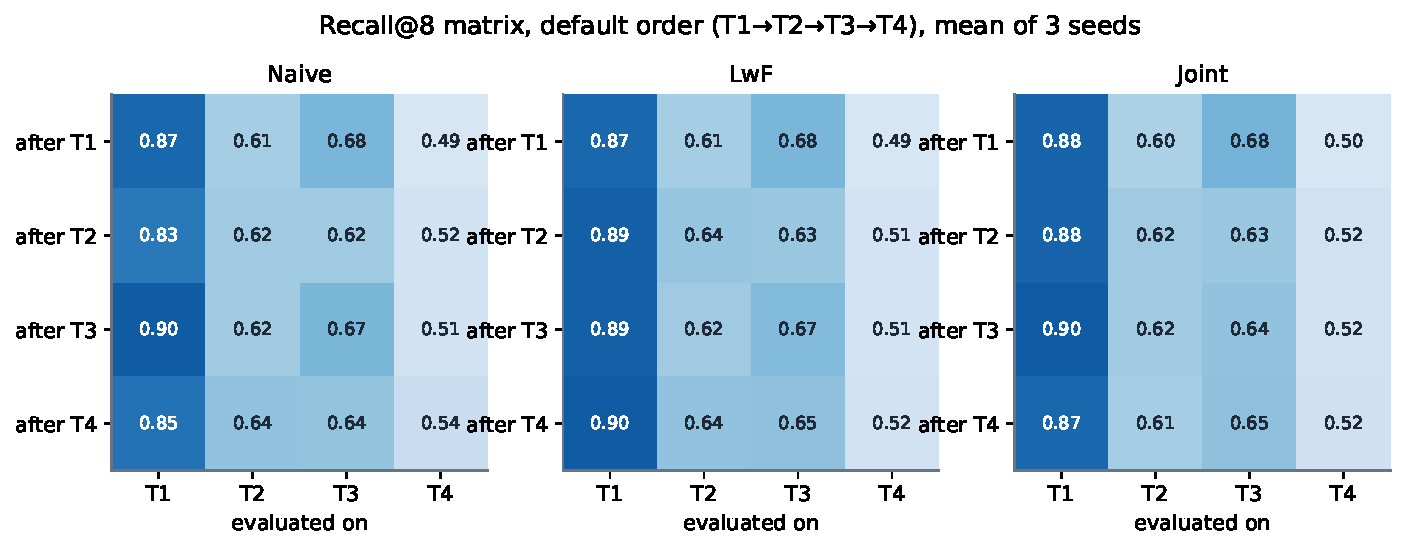
\includegraphics[width=0.92\textwidth]{f11_matrix.pdf}
  \par\small Row $i$: recall on each type after learning the $i$-th type (default order, 3 seeds).
\end{frame}

\begin{frame}{Backup: ACC and FM bars}
  \centering
  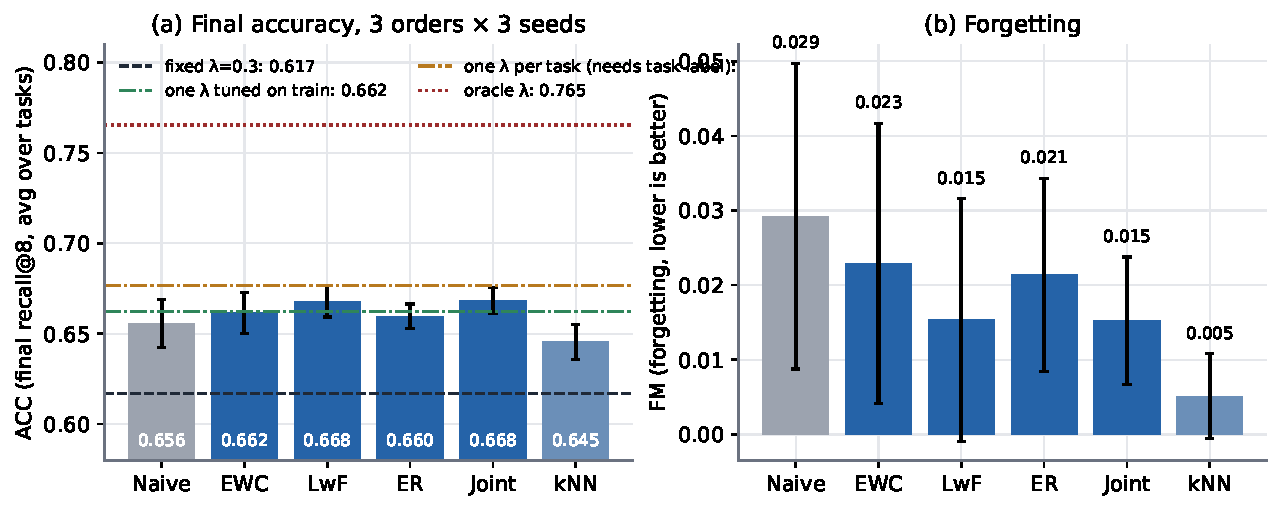
\includegraphics[width=0.9\textwidth]{f09_v4_main.pdf}
\end{frame}

\begin{frame}{Backup: train/test mismatch}
  \centering
  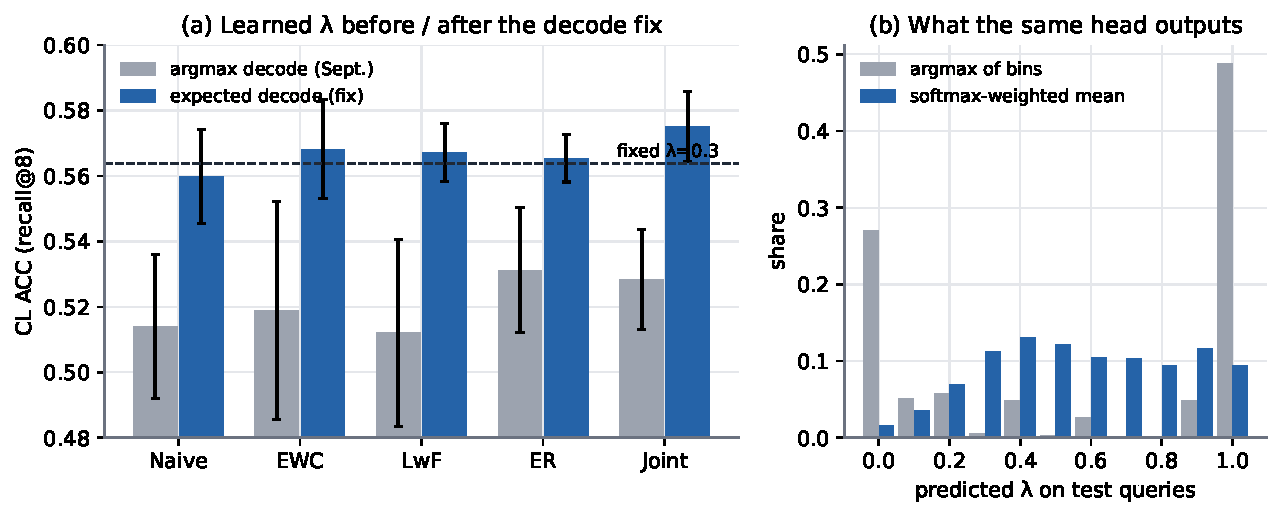
\includegraphics[width=0.85\textwidth]{f05_decode.pdf}
  \par\small Trained on the average $\lam$ but tested on the most likely value, which was 0 or 1. After the fix, learned weights went from 3--5 points below the default to above it.
\end{frame}

\begin{frame}{Backup: which inputs help}
  \centering
  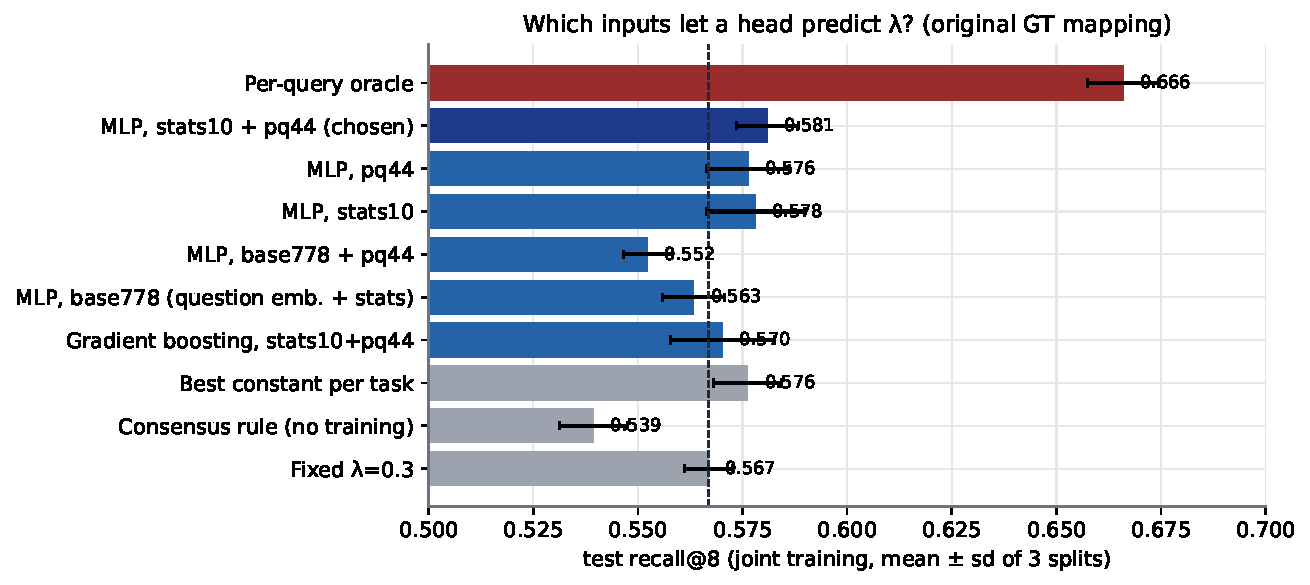
\includegraphics[height=0.72\textheight]{f07_features.pdf}
\end{frame}

\end{document}
